\documentclass[12pt]{article}
\usepackage[paper=letterpaper,margin=2cm]{geometry}
\usepackage{amsmath,amssymb,amsfonts}
\usepackage{newtxtext, newtxmath}
\usepackage{enumitem}
\usepackage{titling}
\usepackage{nicematrix}
\usepackage[colorlinks=true]{hyperref}
\usepackage{graphicx}
\usepackage{listings}
\usepackage{mathtools}

\setlength{\droptitle}{-6em}

\begin{document}

\newcommand{\prob}{\textrm{P}}
\newcommand{\ind}{\perp\!\!\!\!\!\perp} 
\newcommand{\notind}{\not\perp\!\!\!\!\!\perp}
\newcommand{\defeq}{\vcentcolon=}

\center
Aprendizagem 2023\\
Homework III -- Group 016\\
(ist1100293, ist1102556)\vskip 1cm

\large{\textbf{Part I}: Pen and paper}\normalsize

\begin{enumerate}[leftmargin=\labelsep]
    \item Perform one epoch of the EM clustering algorithm and determine the new parameters.
    Hint: we suggest you to use numpy and scipy, however disclose the intermediary results step by step.

    \begin{center}
        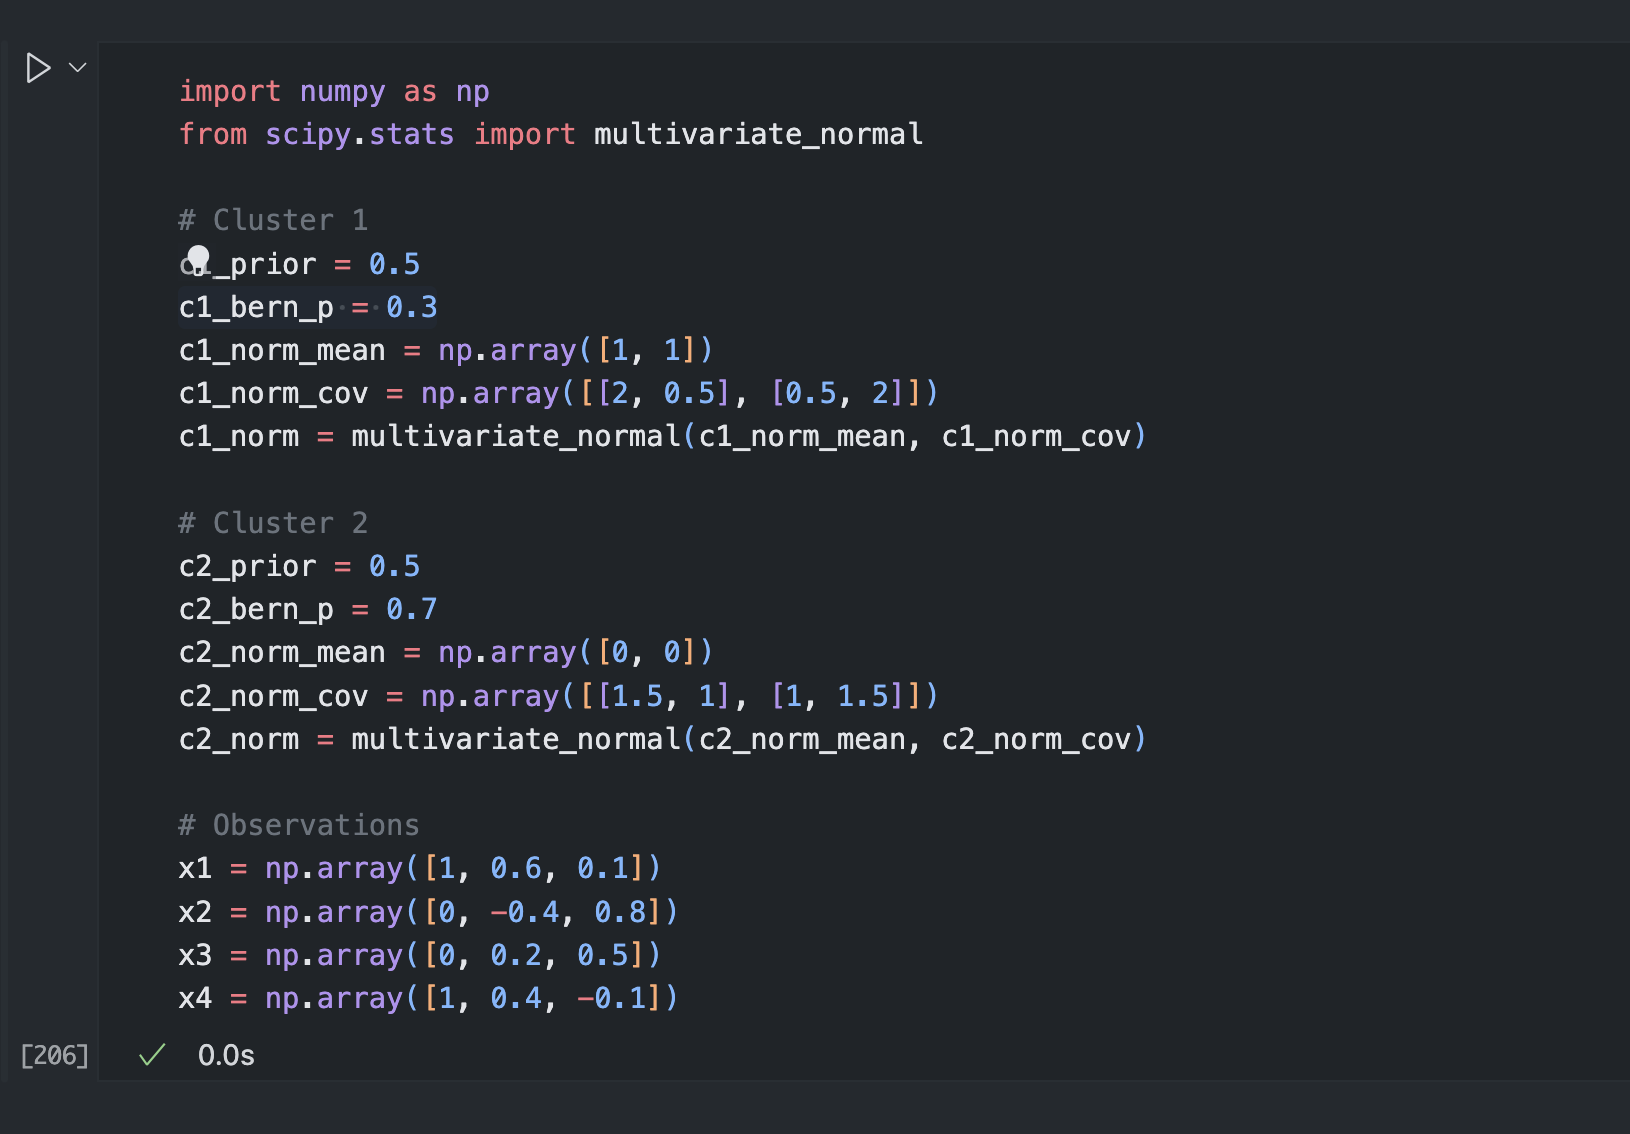
\includegraphics[scale=0.5]{images/code1.png}
    \end{center}

    \paragraph{E-Step} First we will compute the posterior probabilities for each observation for each cluster, with the initial mixture:

    Since $y_1$ is independent from $y_2$ and $y_3$, and follows a Bernoulli distribuition with parameter $p_k$:
    \begin{equation}
    \begin{aligned}
        P(C=c_k|\mathbf{x}) &\propto P(\mathbf{x}|C=c_k)P(C=c_k) \\
        &\propto P(Y_1 = y_1, Y_2 = y_2, Y_3= y_3|C=c_k)P(C=c_k) \\
        &\propto P(Y_1 = y_1|C=c_k)P(Y_2 = y_2, Y_3=y_3|C=c_k)P(C=c_k) \\
        &\propto p_k^{y_1}(1-p_k)^{1-y_1}N_k(y_2, y_3)\pi_k
    \end{aligned}
    \end{equation}

    So, we have:
    \begin{equation}
    \begin{aligned}
        P(C=c_1|\mathbf{x}_1) &\propto p_1N_1(0.6, 0.1)\pi_1 &\qquad P(C=c_2|\mathbf{x}_1) &\propto p_2N_2(0.6, 0.1)\pi_2 \\
        &\propto 0.009986 &\qquad &\propto 0.041866 \\
        P(C=c_1|\mathbf{x}_1) &\approx \frac{0.009986}{0.009986+0.041866} &\qquad P(C=c_2|\mathbf{x}_1) &\approx \frac{0.041866}{0.009986+0.041866} \\
        &\approx 0.1926 &\qquad &\approx 0.8074
    \end{aligned}
    \end{equation}

    \begin{equation}
    \begin{aligned}
        P(C=c_1|\mathbf{x}_2) &\propto (1-p_1)N_1(-0.4, 0.8)\pi_1 &\qquad P(C=c_2|\mathbf{x}_2) &\propto (1-p_2)N_2(-0.4, 0.8)\pi_2 \\
        &\propto 0.017517 &\qquad &\propto 0.010229 \\
        P(C=c_1|\mathbf{x}_2) &\approx \frac{0.017517}{0.017517+0.010229} &\qquad P(C=c_2|\mathbf{x}_2) &\approx \frac{0.010229}{0.017517+0.010229} \\
        &\approx 0.6313 &\qquad &\approx 0.3687
    \end{aligned}
    \end{equation}

    \begin{equation}
    \begin{aligned}
        P(C=c_1|\mathbf{x}_3) &\propto (1-p_1)N_1(0.2, 0.5)\pi_1 &\qquad P(C=c_2|\mathbf{x}_3) &\propto (1-p_2)N_2(0.2, 0.5)\pi_2 \\
        &\propto 0.023931 &\qquad &\propto 0.019437 \\
        P(C=c_1|\mathbf{x}_3) &\approx \frac{0.023931}{0.023931+0.019437} &\qquad P(C=c_2|\mathbf{x}_3) &\approx \frac{0.019437}{0.023931+0.019437} \\
        &\approx 0.5518 &\qquad &\approx 0.4482
    \end{aligned}
    \end{equation}

    \begin{equation}
    \begin{aligned}
        P(C=c_1|\mathbf{x}_4) &\propto p_1N_1(0.4, -0.1)\pi_1 &\qquad P(C=c_2|\mathbf{x}_4) &\propto p_2N_2(0.4, -0.1)\pi_2 \\
        &\propto 0.008857 &\qquad &\propto 0.043575 \\
        P(C=c_1|\mathbf{x}_4) &\approx \frac{0.008857}{0.008857+0.043575} &\qquad P(C=c_2|\mathbf{x}_4) &\approx \frac{0.043575}{0.008857+0.043575} \\
        &\approx 0.1689 &\qquad &\approx 0.8311
    \end{aligned}
    \end{equation}

    \begin{center}
        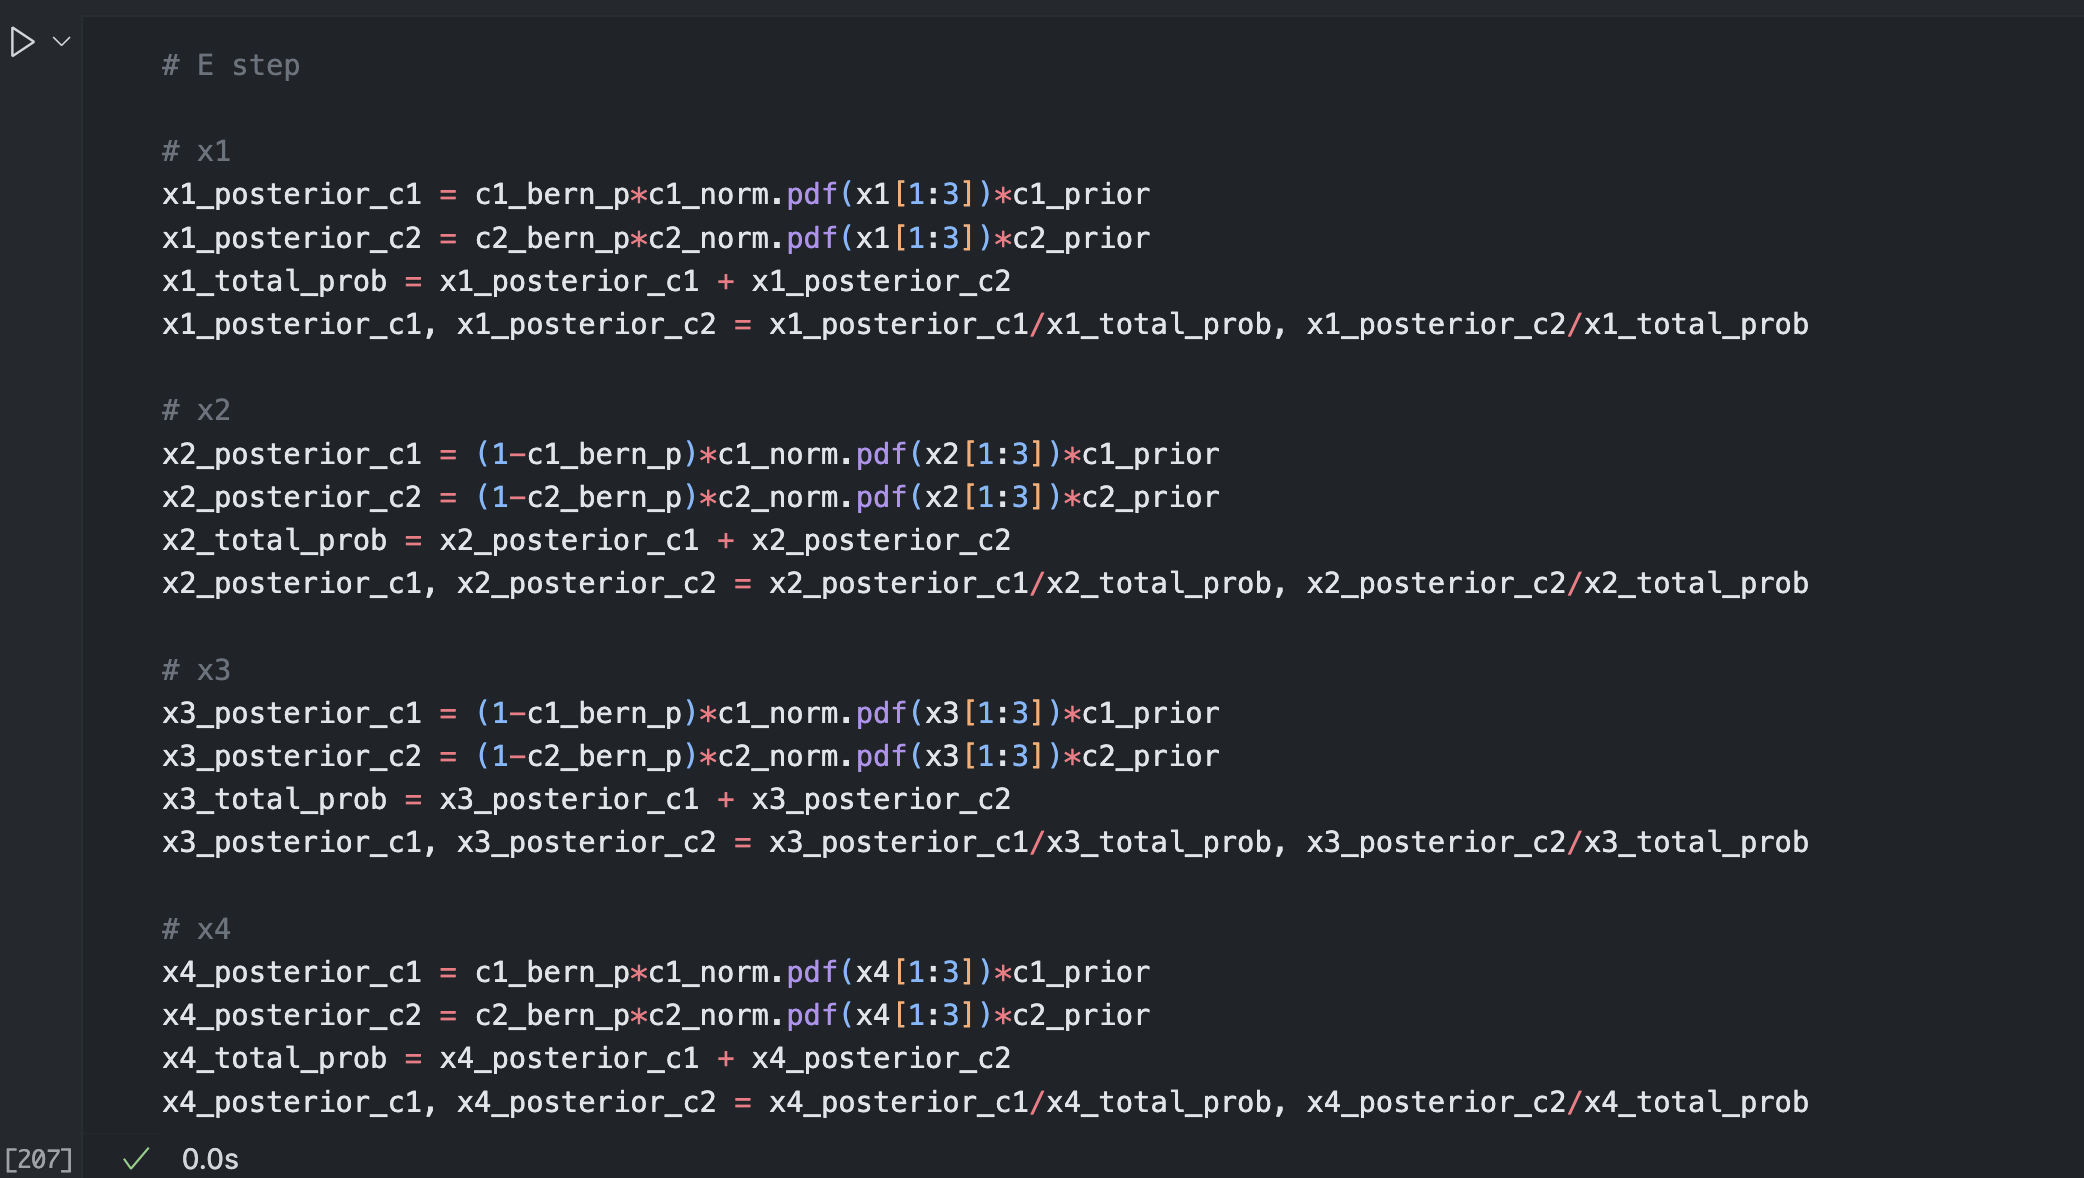
\includegraphics[scale=0.45]{images/code2.png}
    \end{center}
    
    \vskip 4cm

    Using the notation: $\gamma_{ki}=P(C = c_k |\mathbf{x}_i)$. We get:

    \begin{equation}
    \begin{aligned}
        \gamma_{11} = 0.1926 &\qquad \gamma_{21} = 0.8074 \\
        \gamma_{12} = 0.6313 &\qquad \gamma_{22} = 0.3687 \\
        \gamma_{13} = 0.5518 &\qquad \gamma_{23} = 0.4482 \\
        \gamma_{14} = 0.1689 &\qquad \gamma_{24} = 0.8311
    \end{aligned}
    \end{equation}

    \paragraph{M-Step} Now, we need to adjust the cluster parameters. For the normal distribuition, we have:

    \begin{equation}
        \mu_k = \frac{\sum_{i=1}^{n}\gamma_{ki}\mathbf{x}_i}{\sum_{i=1}^{n}\gamma_{ki}} \qquad \Sigma_k = \frac{\sum_{i=1}^{n}\gamma_{ki}(\mathbf{x}_i-\mu_i)(\mathbf{x}_i-\mu_i)^T}{\sum_{i=1}^{n}\gamma_{ki}}
    \end{equation}

    Where $\mathbf{x}_i$ are vectors with only $y_2$ and $y_3$. That gives us:

    \begin{equation}
    \begin{aligned}
        \mu_1 &= \begin{bmatrix}
            0.0265 \\ 0.5071
        \end{bmatrix} &\qquad \mu_2&= \begin{bmatrix}
            0.3091 \\ 0.2104
        \end{bmatrix} \\
        \Sigma_1 &= \begin{bmatrix}
            0.1414  & -0.1054 \\
            -0.1054 & 0.09605 
        \end{bmatrix} &\qquad \Sigma_2 &= \begin{bmatrix}
            0.1083  & -0.0887 \\
            -0.0887 &  0.1041
        \end{bmatrix}
    \end{aligned}
    \end{equation}

    To adjust the parameter of the Bernoulli distribuition, we will use the same estimator as the mean in a normal distribuition.

    \begin{equation}
        p_i = \frac{\sum_{i=1}^{n}\gamma_{ki}x_i}{\sum_{i=1}^{n}\gamma_{ki}}
    \end{equation}

    Where $x_i$ is the $y_1$ variable of the $\mathbf{x}_i$ observation. Which gives us:

    \begin{equation}
    \begin{aligned}
        p_1 = 0.2340 \qquad p_2 = 0.6673
    \end{aligned}
    \end{equation}

    Finally, for the priors, we have:

    \begin{equation}
        \pi_k = \frac{\sum_{i=1}^{N}\gamma_{ki}}{\sum_{j=1}^{N}\sum_{i=1}^{n}\gamma_{ji}}
    \end{equation}

    Which gives us:

    \begin{equation}
        \pi_1 = 0.3862 \qquad \pi_2 = 0.6138
    \end{equation}

    \begin{center}
        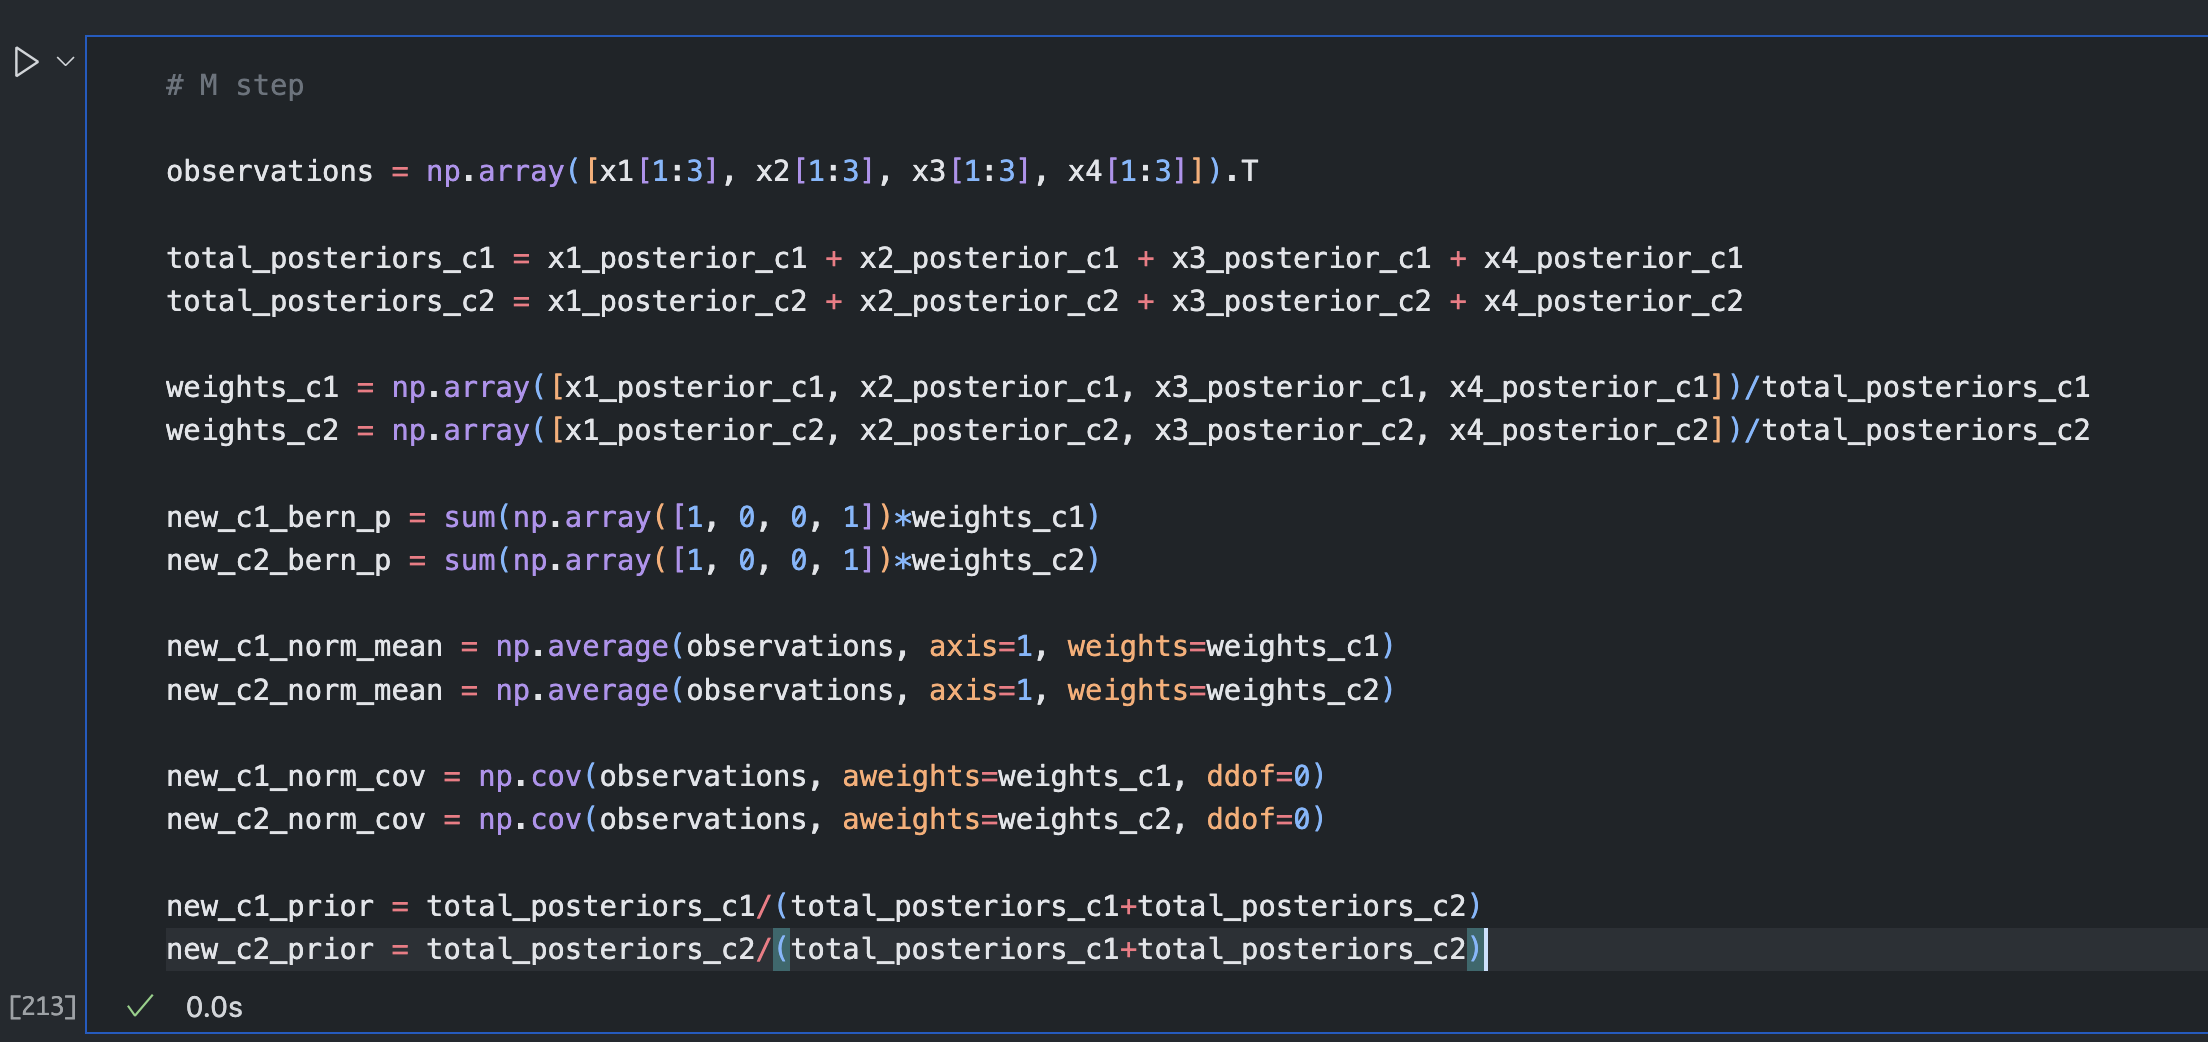
\includegraphics[scale=0.4]{images/code3.png}
    \end{center}

    \item Given the new observation, $\mathbf{x}_{new} = \begin{pmatrix}
        1 \\ 0.3 \\ 0.7 \end{pmatrix}$, determine the cluster memberships (posteriors).

        \begin{equation}
            P(C = c_k | \mathbf{x}_{new}) \propto p_kN_k(0.3, 0.7)\pi_k
        \end{equation}

        \begin{equation}
        \begin{aligned}
            P(C = c_1 | \mathbf{x}_{new}) &= \frac{p_1N_1(0.3, 0.7)\pi_1}{p_1N_1(0.3, 0.7)\pi_1 + p_2N_2(0.3, 0.7)\pi_2} \\
            &\approx 0.0803 \\
            P(C = c_2 | \mathbf{x}_{new}) &= \frac{p_2N_2(0.3, 0.7)\pi_2}{p_1N_1(0.3, 0.7)\pi_1 + p_2N_2(0.3, 0.7)\pi_2} \\
            &\approx 0.9197 \\
        \end{aligned}
        \end{equation}

        \begin{center}
            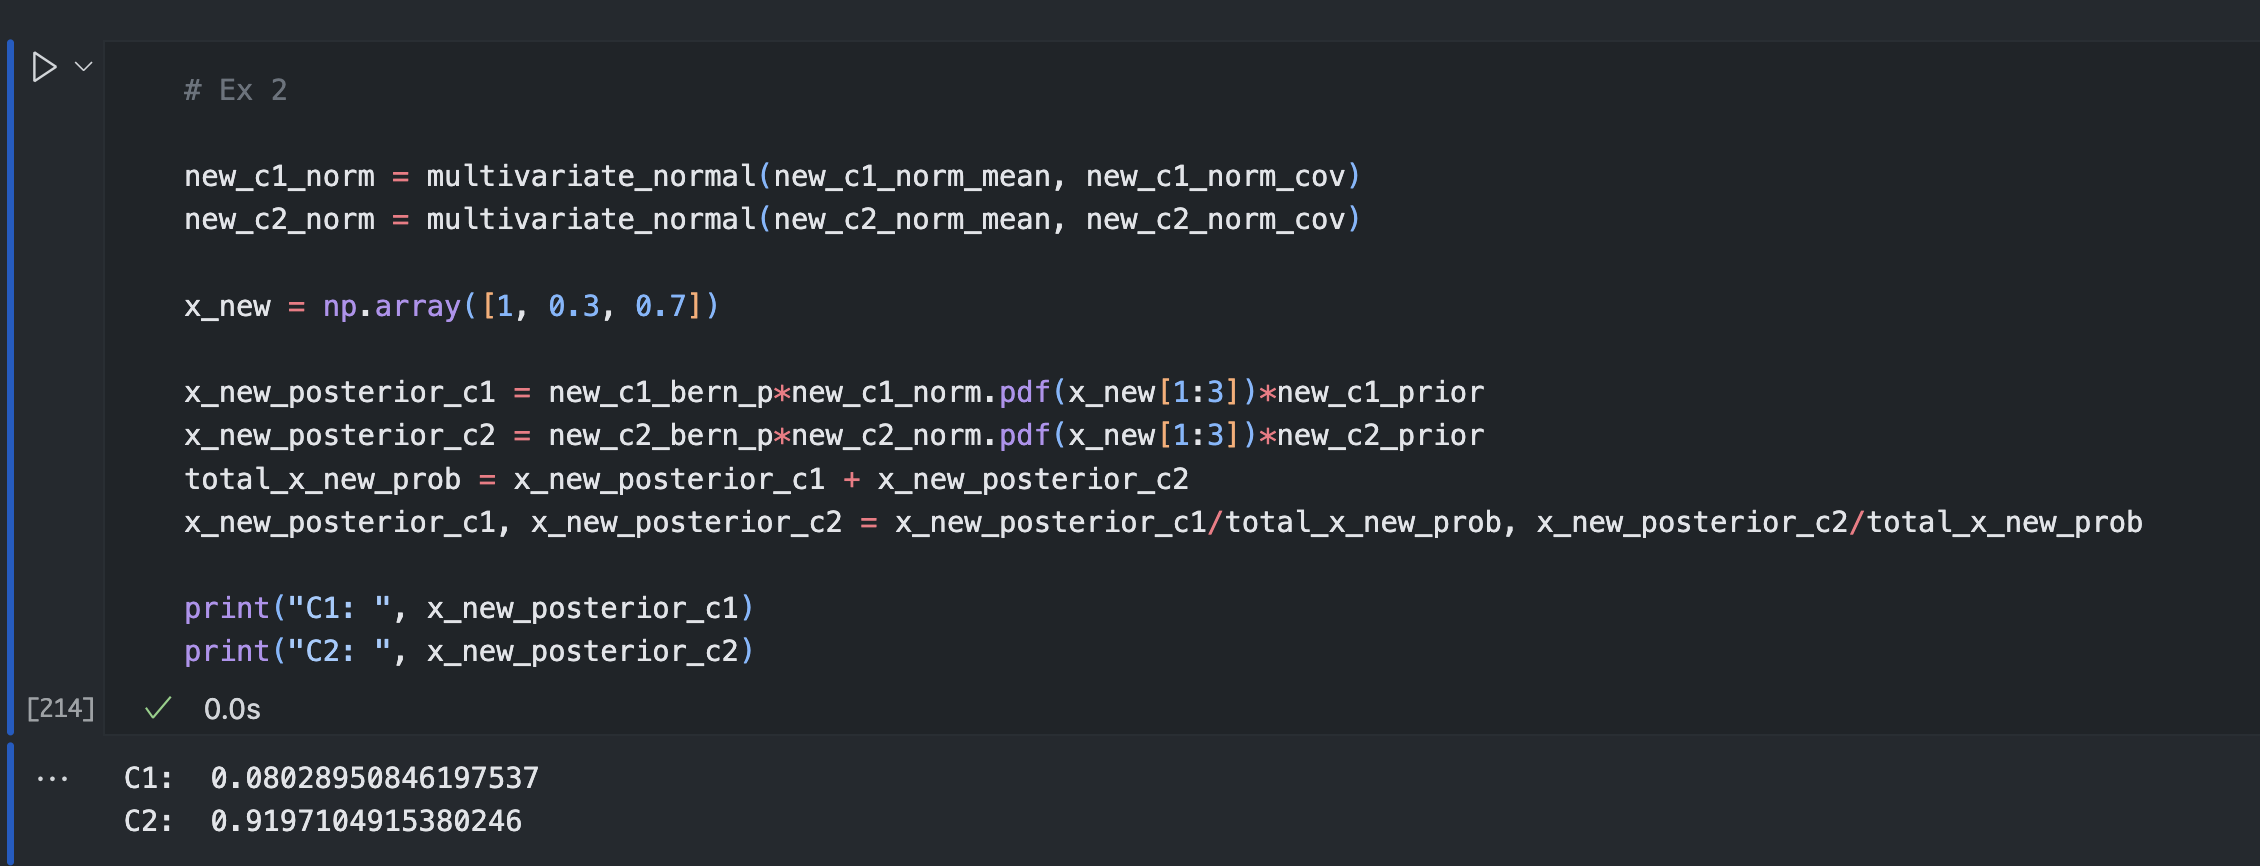
\includegraphics[scale=0.4]{images/code4.png}
        \end{center}
    
    \item Performing a hard assignment of observations to clusters under a ML assumption, identify
    the silhouette of the larger cluster under a Manhattan distance.

    Under a ML assumtion, we will ignore the priors, so:

    \begin{equation}
        P(C = c_k|\mathbf{x}) = P(\mathbf{x}|C = c_k) = p_k^{y_1}(1-p_k)^{y_1}N_k(y_2, y_3)
    \end{equation}

    Also, since we are doing hard assignments, we dont need to normalize these resutls.

    \begin{equation}
    \begin{aligned}
        P(C = c_1 | \mathbf{x}_1) &= 0.2315 &\qquad P(C = c_2 | \mathbf{x}_1) &= 0.9495 \\
        P(C = c_1 | \mathbf{x}_2) &= 1.2663 &\qquad P(C = c_2 | \mathbf{x}_2) &= 0.0887 \\
        P(C = c_1 | \mathbf{x}_3) &= 1.4381 &\qquad P(C = c_2 | \mathbf{x}_3) &= 0.4542 \\
        P(C = c_1 | \mathbf{x}_4) &= 0.0207 &\qquad P(C = c_2 | \mathbf{x}_4) &= 0.7233
    \end{aligned}
    \end{equation}

    \begin{center}
        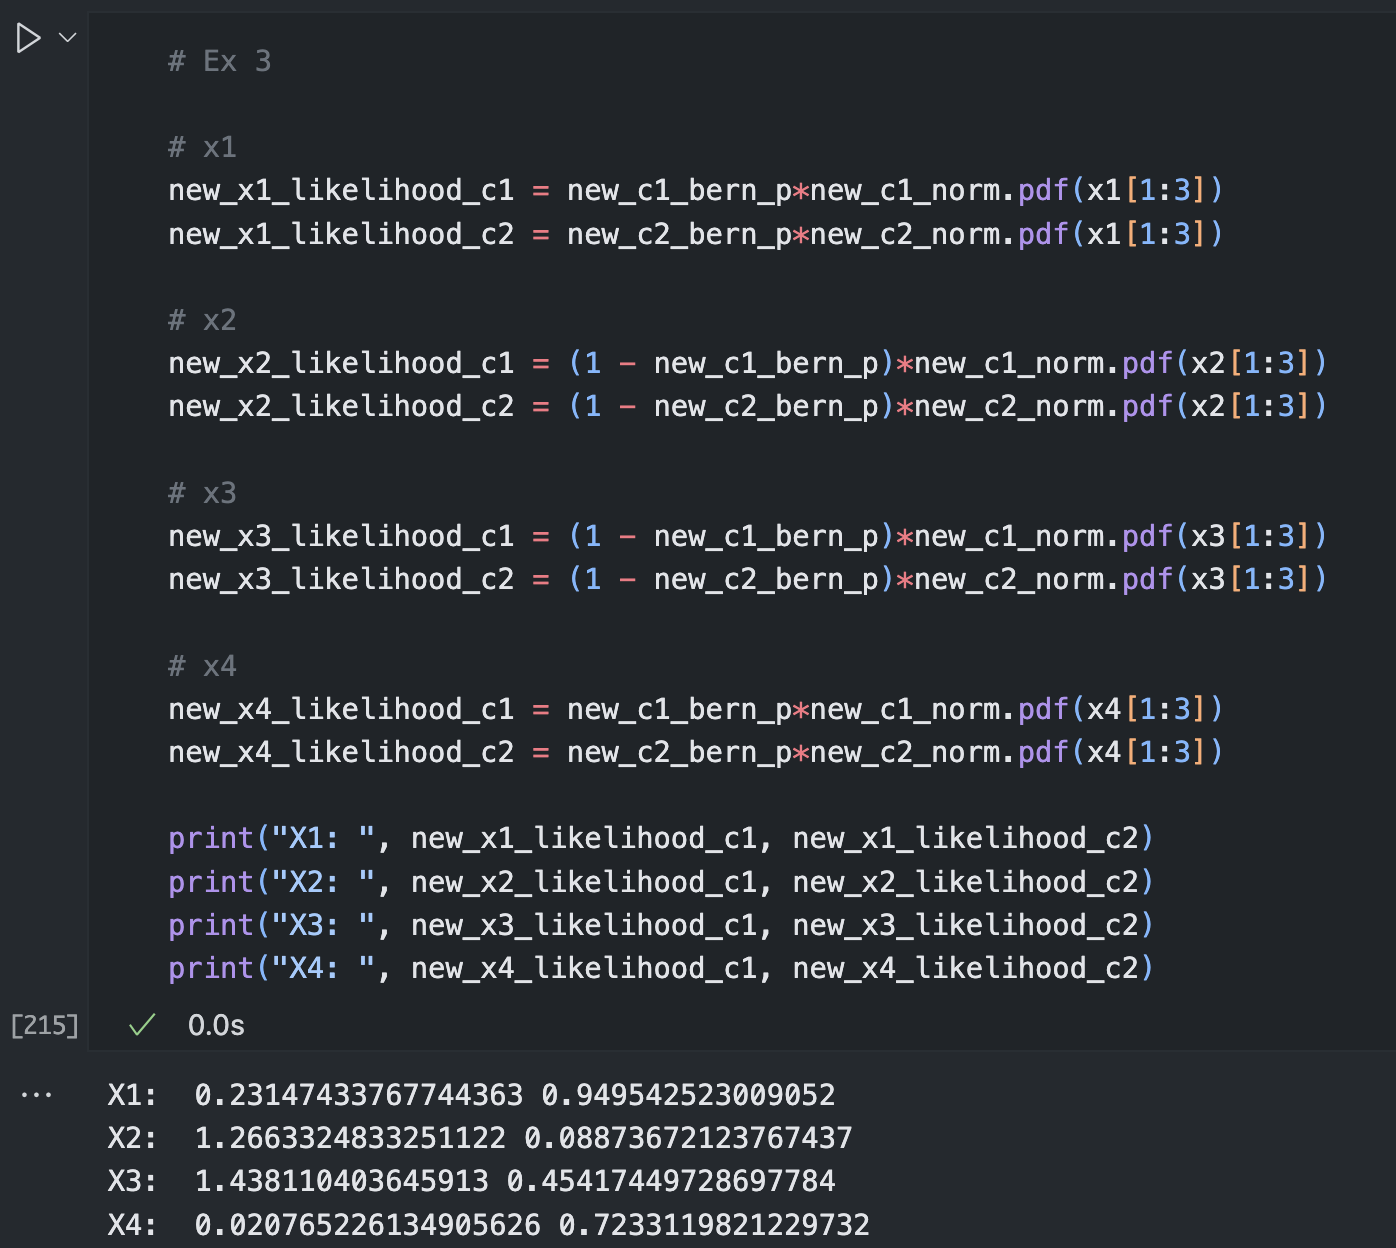
\includegraphics[scale=0.5]{images/code5.png}
    \end{center}

    That way, we can assign $\mathbf{x}_1$, $\mathbf{x}_4$ to $c_1$ and $\mathbf{x}_2$, $\mathbf{x}_3$ to $c_2$.

    Now, to compute the silhouette, we need to compute first the distance between all points:

    \begin{equation}
        d(\mathbf{x}, \mathbf{y}) = |y_1 - x_1| + |y_2 - x_2| + |y_3 - x_3|
    \end{equation}

    \begin{equation}
    \begin{aligned}
        d(\mathbf{x}_1, \mathbf{x}_2) &= 1 + 1   + 0.7 &= 2.7 \\
        d(\mathbf{x}_1, \mathbf{x}_3) &= 1 + 0.4 + 0.4 &= 1.8 \\
        d(\mathbf{x}_1, \mathbf{x}_4) &= 0 + 0.2 + 0.2 &= 0.4 \\
        d(\mathbf{x}_2, \mathbf{x}_3) &= 0 + 0.6 + 0.3 &= 0.9 \\
        d(\mathbf{x}_2, \mathbf{x}_4) &= 1 + 0.8 + 0.9 &= 2.7 \\
        d(\mathbf{x}_3, \mathbf{x}_4) &= 1 + 0.2 + 0.6 &= 1.8
    \end{aligned}
    \end{equation}

    Then, the silhouette of a single point will be:
    \begin{equation}
        s(\mathbf{x}_i) = 1 - \frac{a(\mathbf{x}_i)}{b(\mathbf{x}_i)}
    \end{equation}

    Where $a(\mathbf{x})$ is the average distance from $\mathbf{x}$ to the other members of it's cluster, and $b(\mathbf{x})$ is the maximum of the average distance to the members of other cluster.

    \begin{equation}
    \begin{aligned}
        s(\mathbf{x}_1) &= 1 - \frac{0.4}{\frac{1}{2}(2.7+1.8)} = 0.8222 \\
        s(\mathbf{x}_2) &= 1 - \frac{0.9}{\frac{1}{2}(2.7+2.7)} = 0.6667 \\
        s(\mathbf{x}_3) &= 1 - \frac{0.9}{\frac{1}{2}(1.8+1.8)} = 0.5 \\
        s(\mathbf{x}_4) &= 1 - \frac{0.4}{\frac{1}{2}(2.7+1.8)} = 0.8222
    \end{aligned}
    \end{equation}

    Now, the silhouette for the clusters is the average silhouette of it's members:

    \begin{equation}
    \begin{aligned}
        s(c_1) = \frac{s(\mathbf{x}_2) + s(\mathbf{x}_3)}{2} = 0.5833 \\
        s(c_2) = \frac{s(\mathbf{x}_1) + s(\mathbf{x}_4)}{2} = 0.8222
    \end{aligned}
    \end{equation}

    \item Knowing the purity of the clustering solution is 0.75, identify the number of possible classes
    (ground truth).

    With the purity definition:

    \begin{equation}
        purity = \frac{1}{n} \sum_{k=1}^{K} \max_j(|C_k \cap L_j|)
    \end{equation}

    By inputing the known values, we get:

    \begin{equation}
    \begin{aligned}
        \frac{1}{4}(\max_j(|C_1 \cap L_j|) + \max_j(|C_2 \cap L_j|)) &= 0.75 \\
        \max_j(|C_1 \cap L_j|) + \max_j(|C_2 \cap L_j|) &= 3
    \end{aligned}
    \end{equation}

    Since $|C_1|$ and $|C_2|$ are both $2$, both of the parcels will have a maximum value of 2. The parcels also will have a minimum value of $1$. That way, for the sum to equal $3$, one of them needs to be $1$ and the other $2$. That means that for one of the clusters, both of the observations need to belong to the same class, while for the other cluster, each observation needs to belong to a different class. That means that, if we assume that all classes are represented in the data, there can either be $2$ or $3$ distinct classes. That depends if the class of the two elements of the same cluster is also represented on the other cluster, or not.
\end{enumerate}

\vskip 10cm

\large{\textbf{Part II}: Programming and Critical Analysis}\normalsize

Recall the column\_diagnosis.arff dataset from previous homeworks. For the following exercises,
normalize the data using sklearn's MinMaxScaler.

\begin{center}
    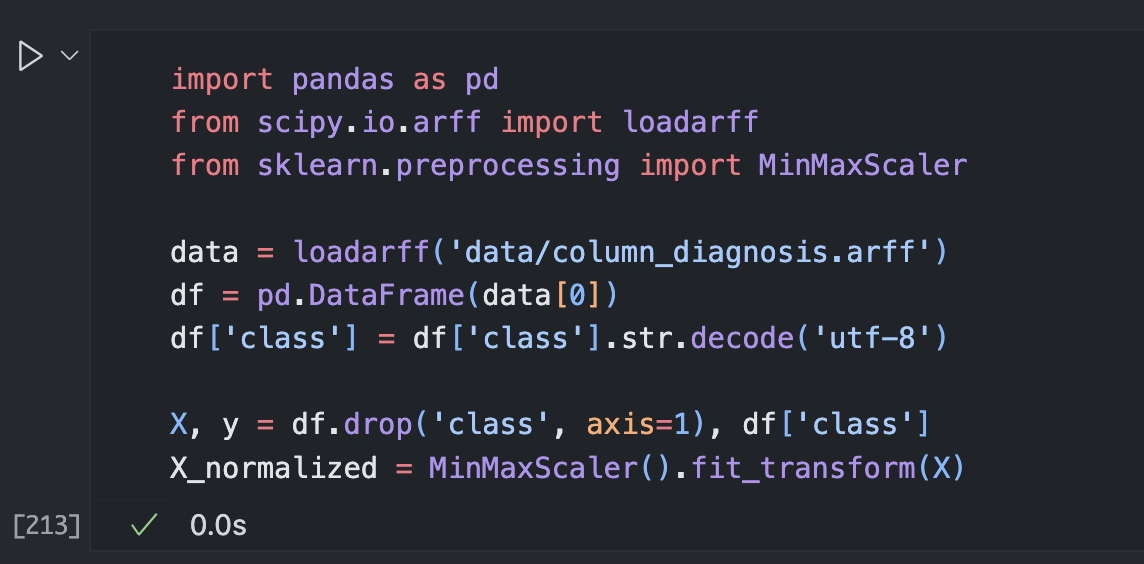
\includegraphics[scale=0.5]{images/code6.png}
\end{center}

\begin{enumerate}
    \item Using sklearn, apply k-means clustering fully unsupervisedly on the normalized data with
    $k \in \{2,3,4,5\}$ (random=0 and remaining parameters as default). Assess the silhouette and purity of
    the produced solutions.

    \begin{center}
        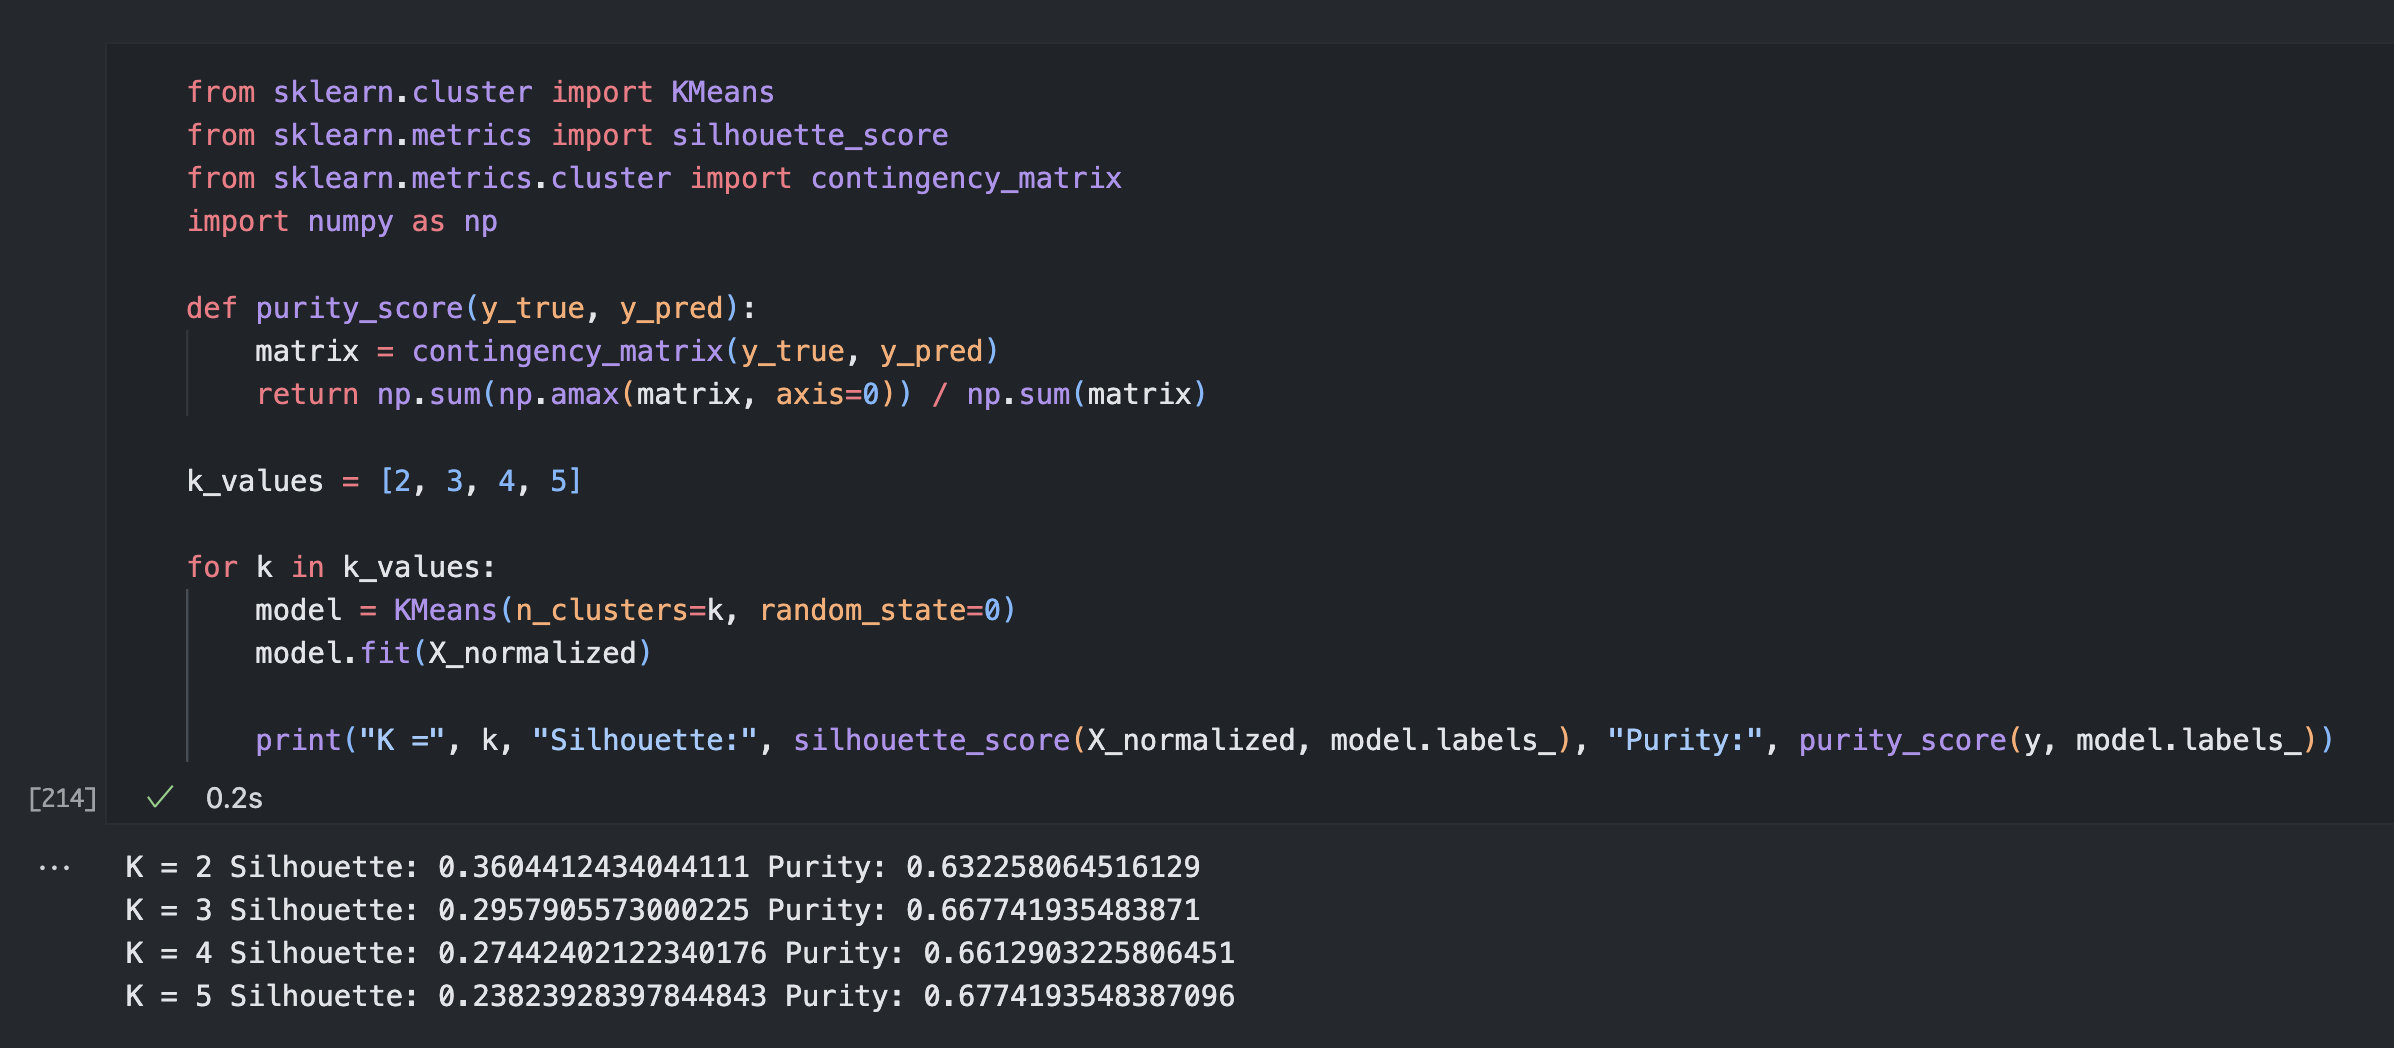
\includegraphics[scale=0.38]{images/code7.png}
    \end{center}

    \item Consider the application of PCA after the data normalization:
    
    \begin{center}
        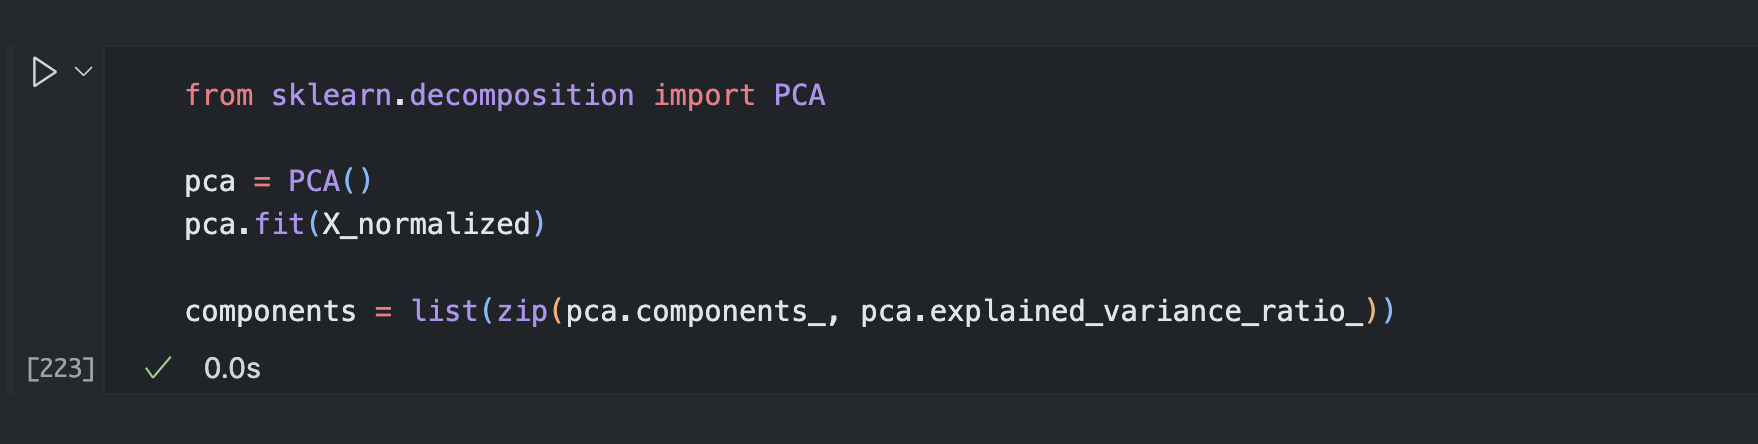
\includegraphics[scale=0.5]{images/code8.png}
    \end{center}

    \begin{enumerate}
        \item Identify the variability explained by the top two principal components.
            \begin{center}
                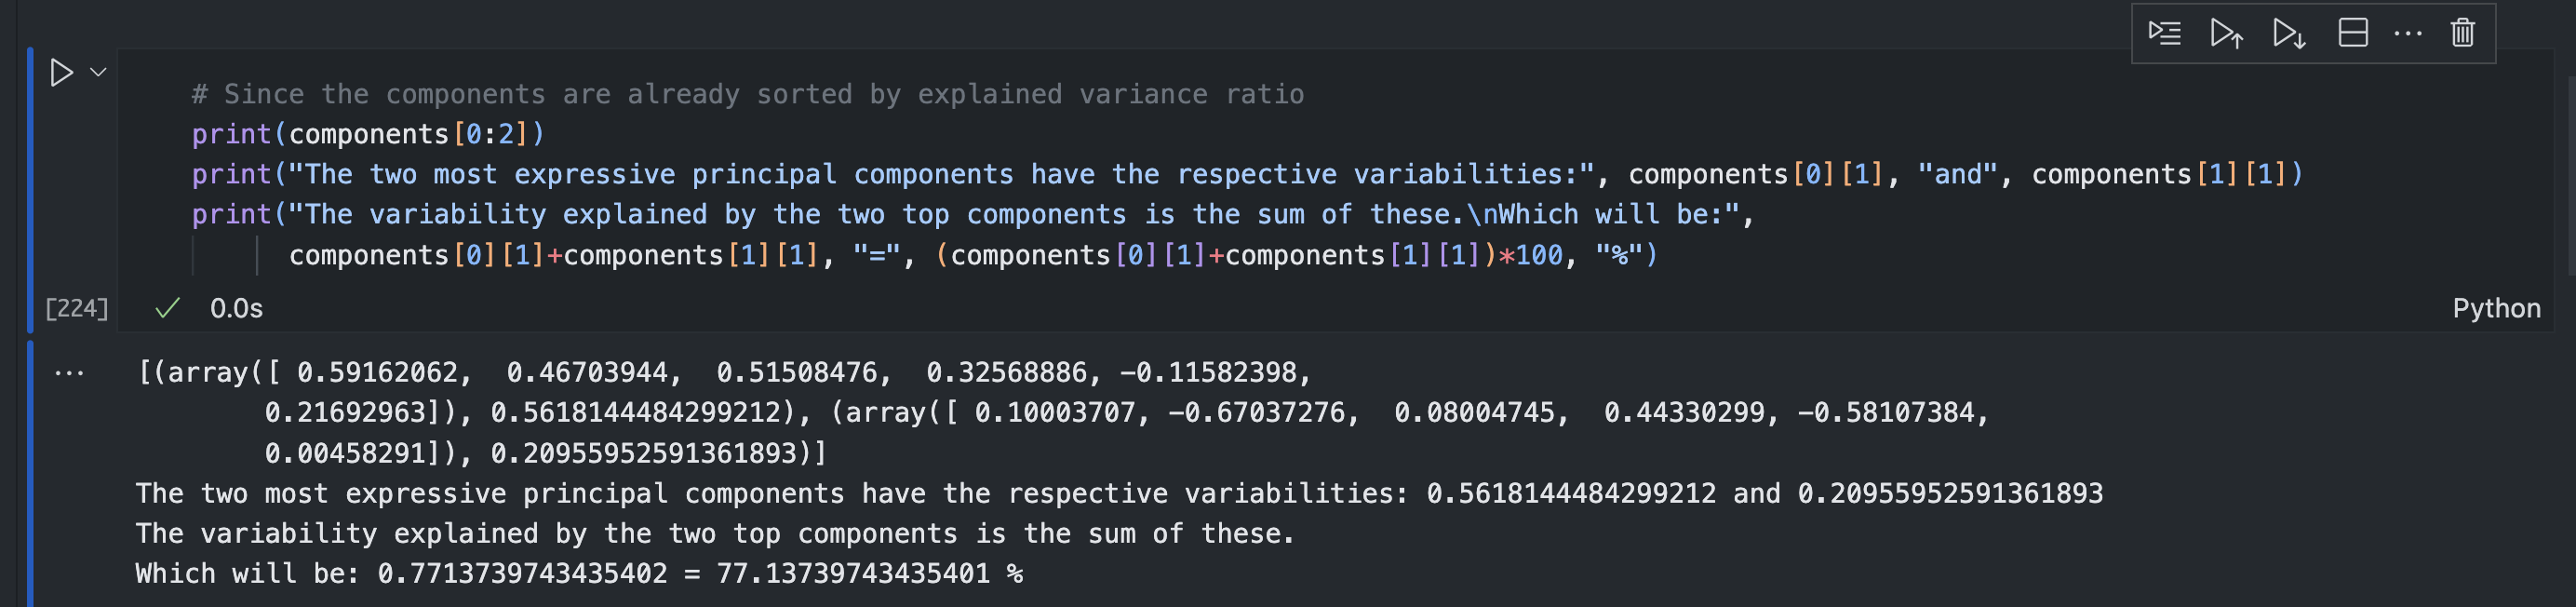
\includegraphics[scale=0.3]{images/code9.png}
            \end{center}
        
        \item For each one of these two components, sort the input variables by relevance by
        inspecting the absolute weights of the linear projection.
    
        \begin{center}
            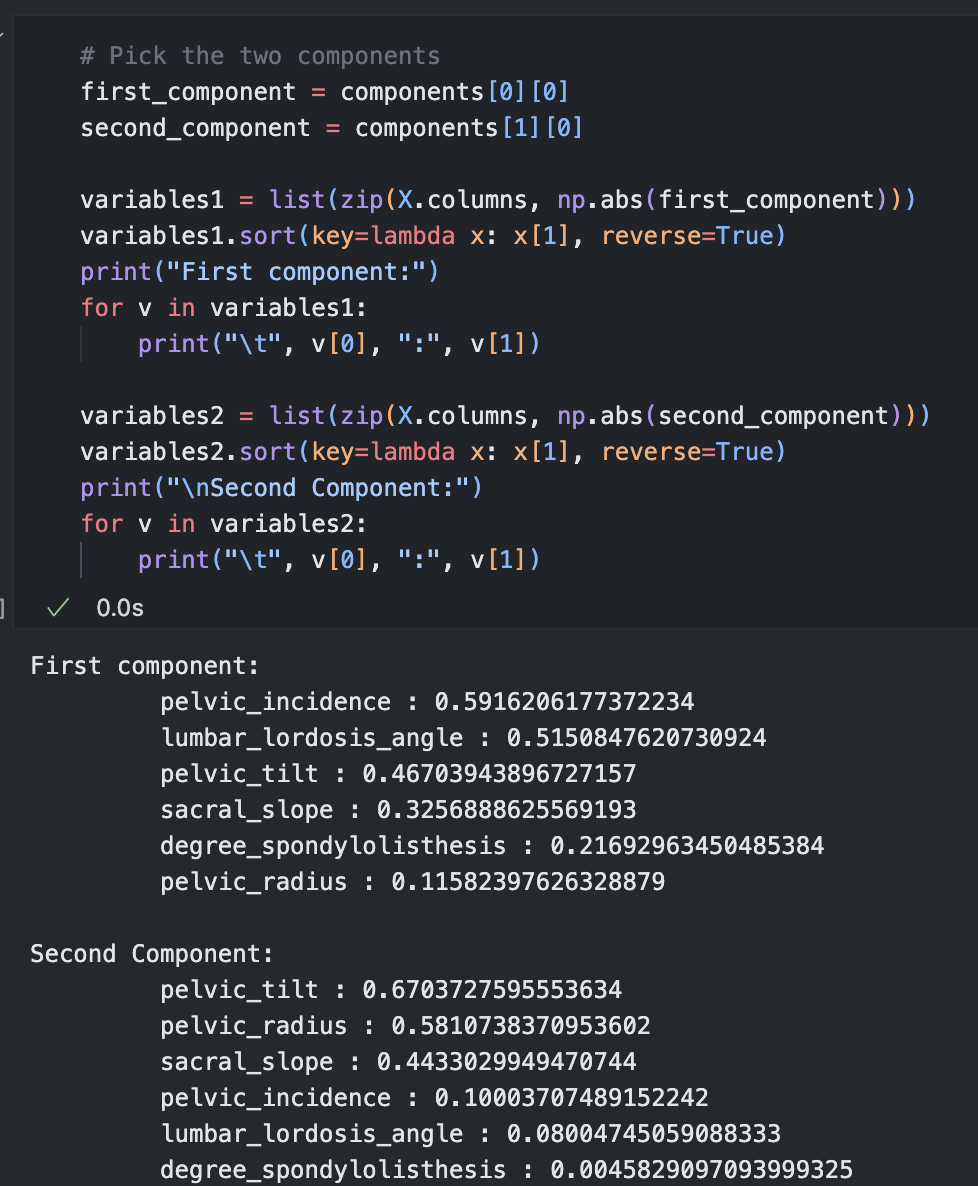
\includegraphics[scale=0.6]{images/code10.png}
        \end{center}
    \end{enumerate}

    \item Visualize side-by-side the data using: i) the ground diagnoses, and ii) the previously learned
    $k = 3$ clustering solution. To this end, projected the normalized data onto a 2-dimensional data
    space using PCA and then color observations using the reference and cluster annotations

    \begin{center}
        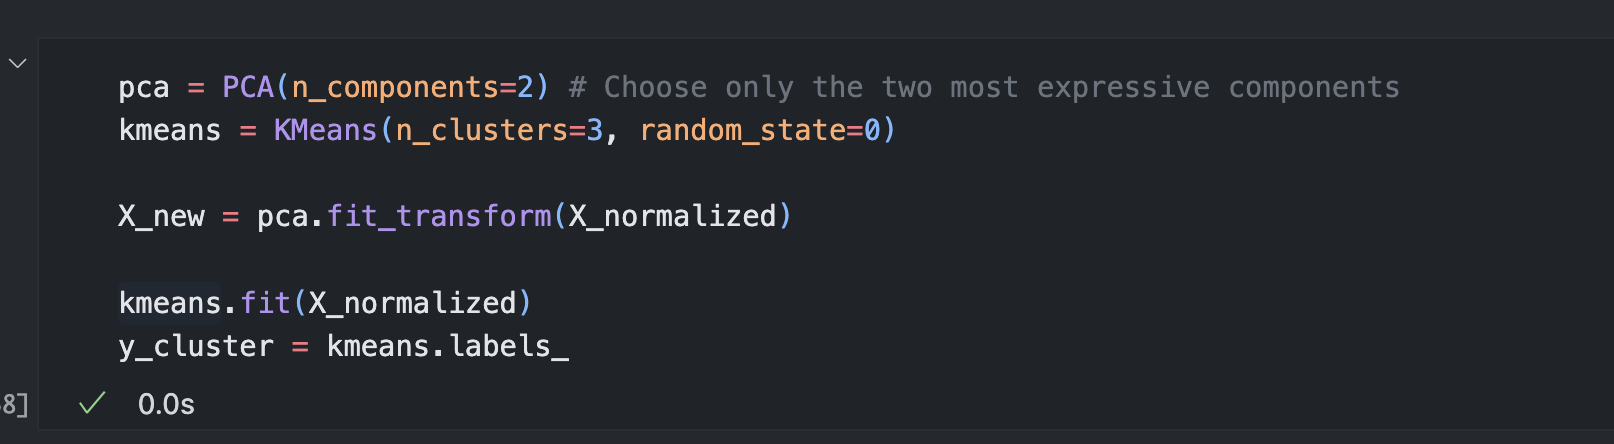
\includegraphics[scale=0.5]{images/code11.png}
    \end{center}

    \begin{center}
        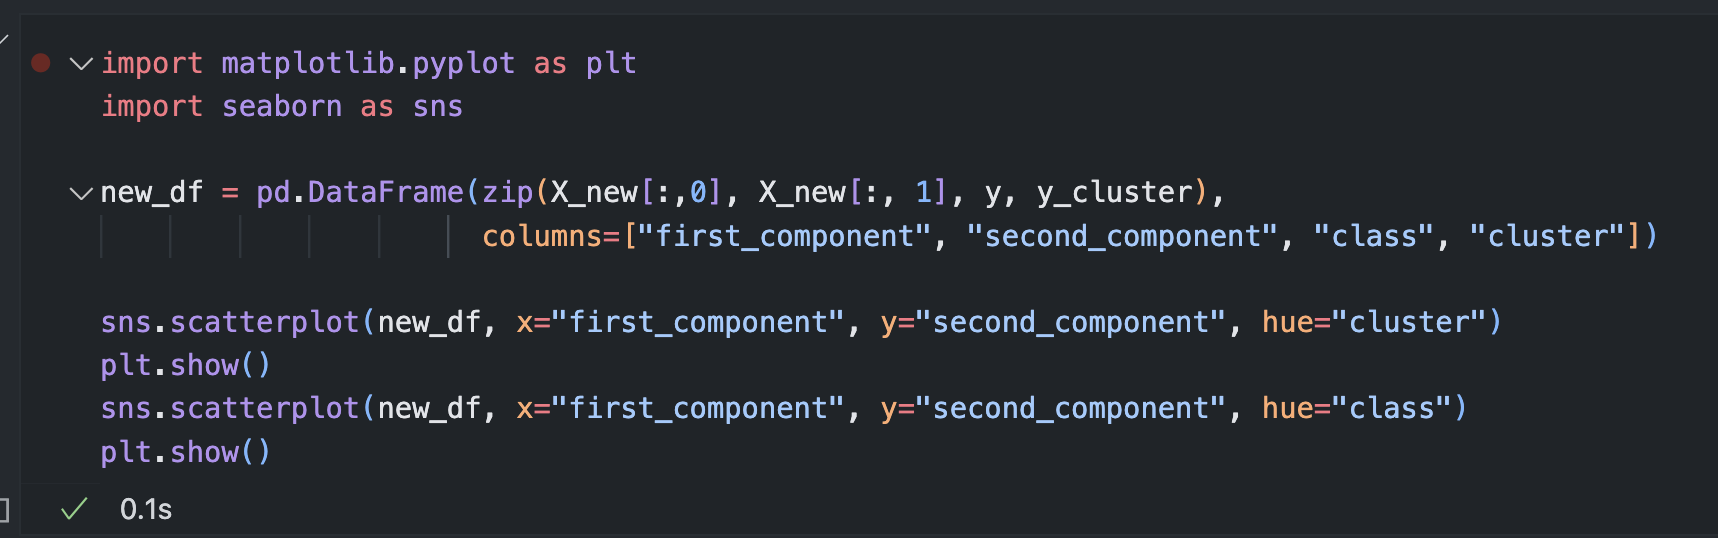
\includegraphics[scale=0.5]{images/code12.png}
    \end{center}

    \paragraph{Results:}

    \begin{center}
        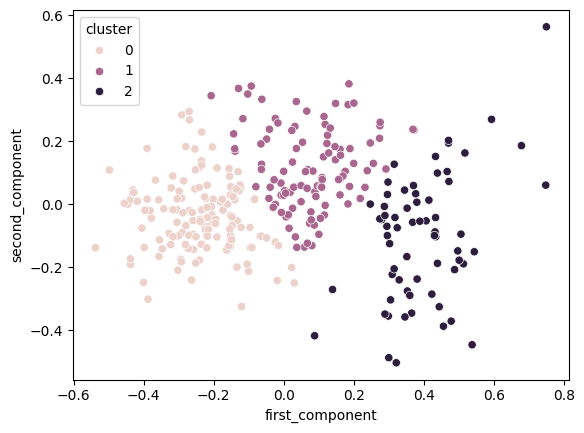
\includegraphics[scale=0.5]{images/graph1.png}
    \end{center}

    \begin{center}
        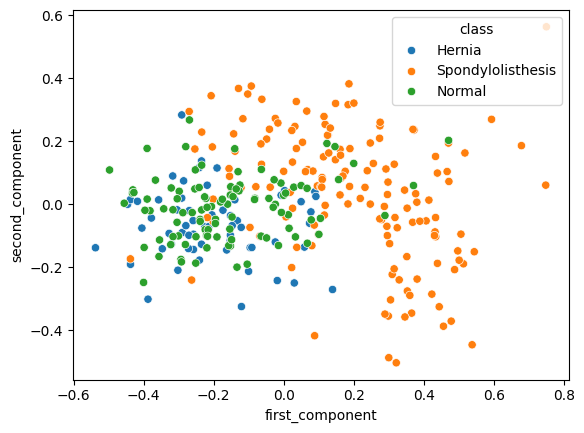
\includegraphics[scale=0.5]{images/graph2.png}
    \end{center}

    \item Considering the results from questions (1) and (3), identify two ways on how clustering can
    be used to characterize the population of ill and healthy individuals.

    Given a clustering model that was trained with our data, we can use this cluster information in two ways that allow us to describe each condition. If our model's purity is high, we can hard-assign each cluster to a condition. That way, each condition can be seen as a set of groups, each with people with similar characteristics. However, if we can't get a model with good purity, we can analyze graphically the plot of our observations by using a dimensionality reduction technique. That way, we can observe geometrically the properties of each class (in this case, each condition) and each cluster. By relating those two, we can characterize our population. This method gets easier if the clustering model has high silhouette, since the clusters will be more cohese and separate (between each other).
\end{enumerate}

\end{document}
